% !TeX program = xelatex
\documentclass{article}
\usepackage{kotex}
\usepackage[a4paper, left=3cm, right=3cm, top=2.5cm, bottom=2.5cm]{geometry}
\usepackage{amsmath, amssymb}
\usepackage{tcolorbox}
\usepackage{caption}
\usepackage{setspace}
\usepackage{xcolor}
\usepackage{titlesec}
\usepackage{enumerate}
\usepackage{tikz}
\usetikzlibrary{arrows.meta, calc}

\setstretch{1.3}
\renewcommand{\figurename}{그림}
\titleformat{name=\section,numberless}
  {\normalfont\large\bfseries\color{blue}}{}
  {0pt}{}

\title{2.6 각에 대한 코사인 법칙}
\date{}
\author{}

\begin{document}
\maketitle

\section*{2.6 각에 대한 코사인 법칙}

다음 결과는 쌍대성을 사용하여 변에 대한 코사인 법칙으로부터 바로 얻을 수 있다.

\begin{tcolorbox}[
  colback=red!4, colframe=red!60!black,
  title=따름정리 2.6.1 (각에 대한 코사인 법칙),
  fonttitle=\bfseries, boxrule=0.5mm, arc=3mm]

$\triangle ABC$를 구면 삼각형이라 하고 $A$의 대변을 $a$, $B$의 대변을 $b$, $C$의 대변을 $c$라 하자.
그러면 다음이 성립한다.
\begin{equation}
  \cos\angle A = -\cos\angle B\cos\angle C + \sin\angle B\sin\angle C\cos\angle a
  \tag{2.18}
\end{equation}

\end{tcolorbox}

\textbf{증명.}\quad
쌍대 삼각형 $\triangle A^*B^*C^* = {}^*\!\triangle ABC$에 변에 대한 코사인 법칙(정리 2.4.1)을 적용하면 다음을 얻는다.
\begin{equation}
  \cos\angle a^* = \cos\angle b^*\cos\angle c^* + \sin\angle b^*\sin\angle c^*\cos\angle A^*
  \tag{2.19}
\end{equation}
여기서 $a^*$는 $A^*$의 대변, $b^*$는 $B^*$의 대변, $c^*$는 $C^*$의 대변이다.
따름정리 2.5.3으로부터
$\angle a^* = 180° - \angle A$, $\angle b^* = 180° - \angle B$, $\angle c^* = 180° - \angle C$이다.
이를 식 (2.19)에 대입하고 임의의 각 $\theta$에 대해
$\cos(180°-\theta) = -\cos\theta$, $\sin(180°-\theta) = \sin\theta$를 사용하면 식 (2.18)을 얻는다.
\hfill $\square$

\medskip
세 꼭짓각이 주어지면 구면 삼각형은 완전하게 풀린다.
그러므로 두 구면 삼각형의 세 꼭짓각이 각각 동일하면 두 삼각형은 합동이다.
평면 기하에서는 두 삼각형의 세 각이 일치하면 두 삼각형은 단지 닮은 삼각형일 뿐이다.

\bigskip
\textbf{보기 2.6.1}\quad
구면 삼각형의 세 꼭짓각이 $\angle A = 60°$, $\angle B = 70°$, $\angle C = 80°$일 때
세 호각 $\angle a$, $\angle b$, $\angle c$를 구하여라.

\medskip
\textbf{풀이.}\quad
각에 대한 코사인 법칙으로부터 다음을 얻는다.
\begin{align*}
  \cos\angle a
  &= \frac{\cos\angle A + \cos\angle B\cos\angle C}{\sin\angle B\sin\angle C}
   \approx \frac{.50000 + (.34202)(.17365)}{(.93969)(.98481)} \\
  &\approx .60447
\end{align*}
이로부터 $\angle a$는 다음과 같다.
\[
  \angle a \approx \arccos(.60447) \approx 52.809°
\]
같은 방법으로 계산하면 다음과 같다.
\begin{align*}
  \cos\angle b
  &= \frac{\cos 70° + \cos 60°\cos 80°}{\sin 60°\sin 80°}
   \approx \frac{.34202 + (.50000)(.17365)}{(.86603)(.98481)} \\
  &\approx .50283 \\[6pt]
  \cos\angle c
  &= \frac{\cos 80° + \cos 60°\cos 70°}{\sin 60°\sin 70°}
   \approx \frac{.17365 + (.50000)(.34202)}{(.86603)(.93969)} \\
  &\approx .42353
\end{align*}
따라서 다음을 얻는다.
\[
  \angle b \approx 59.813°,\qquad \angle c \approx 64.943°
\]
\hfill $\square$

\medskip
구면에서 동일한 꼭짓점을 갖는 각들을 결합하면 각은 평면에서처럼 더해진다.
예를 들어 그림 2.13에서 $\angle a + \angle b + \angle c = 360°$이다.
그 이유는 구면에서 두 곡선 사이의 각은, 정의에 의해, 곡선의 접선 사이의 각과 같기 때문이다.
따라서 여러 각이 동일한 꼭짓점을 가지면 이들 각은 한 접평면에서 벡터들 사이의 각처럼 결합한다.

\begin{figure}[ht]
\centering
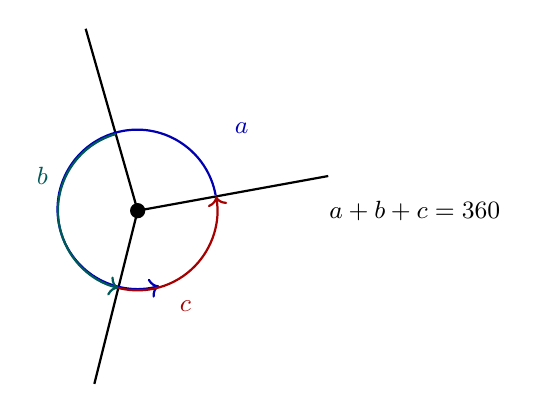
\begin{tikzpicture}[scale=1.1]
  % Central vertex
  \fill (0,0) circle (2.5pt);
  % Three arcs (lines) meeting at center
  \draw[thick] (0,0) -- (2.2, 0.4);
  \draw[thick] (0,0) -- (-0.6, 2.1);
  \draw[thick] (0,0) -- (-0.5, -2.0);
  % Angle arcs
  \draw[->, thick, blue!70!black]
    (0.9, 0.18) arc ({atan(0.4/2.2)}:{atan(2.1/-0.6)+360}:0.92cm);
  \draw[->, thick, red!65!black]
    ({-0.5*0.92/sqrt(0.25+4.0)}, {-2.0*0.92/sqrt(0.25+4.0)})
      arc ({atan(-2.0/-0.5)+180}:{atan(0.4/2.2)+360}:0.92cm);
  \draw[->, thick, teal!70!black]
    ({-0.6*0.92/sqrt(0.36+4.41)}, {2.1*0.92/sqrt(0.36+4.41)})
      arc ({atan(2.1/-0.6)+180}:{atan(-2.0/-0.5)+180}:0.92cm);
  % Labels for angles
  \node[blue!70!black,  font=\small] at (1.2, 0.95) {$a$};
  \node[teal!70!black,  font=\small] at (-1.1, 0.4) {$b$};
  \node[red!65!black,   font=\small] at (0.55,-1.1) {$c$};
  % Label for sum
  \node[font=\small] at (3.2, 0) {$a+b+c = 360°$};
\end{tikzpicture}
\caption{한 꼭짓점에서 세 각의 합 (그림 2.13)}
\label{fig:2.13}
\end{figure}

\bigskip
\textbf{보기 2.6.2}\quad
정십이면체는 대칭인 닫힌 곡면으로 열두 개의 합동인 정오각형을 각 꼭짓점에서
세 개씩 모이도록 변을 따라 붙인 것이다(그림 2.14).
각 변의 길이가 $10\,\text{cm}$일 때 정십이면체의 꼭짓점에서 중심까지의 거리를 구하여라.

\medskip
\textbf{풀이.}\quad
정십이면체에서 $A$와 $B$를 인접한 꼭짓점이라 하고 중심을 $O$라 하자.
$\angle AOB$의 크기를 알면 $\triangle AOB$를 풀어서, 즉 다음과 같이 평면의 삼각형에 대한
코사인 법칙을 사용하여 길이 $OA$를 알아낼 수 있다.
\begin{equation}
  (10\,\text{cm})^2 = 2(OA)^2 - 2(OA)^2\cos\angle AOB
  \tag{2.20}
\end{equation}

구면 삼각형을 풀어서 $\angle AOB$를 구해보자.
정십이면체를 외접구에 사영시키면 열두 개의 합동인 ``구면 오각형''으로 이루어진 구면을 얻는다.
그런 다음 각 구면 오각형을 그 중심과 꼭짓점을 이어서 다섯 개의 이등변 구면 삼각형으로 나눈다
(그림 2.14 참조).
$C$를 한 구면 오각형의 중심이라 하고 $\triangle ABC$를 얻은 삼각형 중 하나라고 하자.
각 꼭짓점에서 세 개의 구면 오각형이 모이므로 구면 오각형의 각은
$360°/3 = 120°$로 계산된다.
오각형의 내부에서는 두 개의 삼각형이 각 꼭짓점에 모이기 때문에 다음을 얻는다.
\[
  \angle A = \angle B = \frac{120°}{2} = 60°
\]
다섯 개의 삼각형이 오각형의 중심에서 만나므로 다음을 얻는다.
\[
  \angle C = \frac{360°}{5} = 72°
\]
이를 각에 대한 코사인 법칙에 적용하면 다음과 같다.
\[
  \cos\angle\widehat{AB}
  = \frac{\cos 72° + \cos^2 60°}{\sin^2 60°}
  \approx 0.74536
\]
따라서 식 (2.20)에 의해 다음을 얻는다.
\[
  OA \approx \frac{10\,\text{cm}}{\sqrt{2 - 2(0.74536)}} = 14.01\,\text{cm}
\]
\hfill $\square$

\begin{figure}[ht]
\centering
\begin{tikzpicture}[scale=0.88]
  %--- (1) 정십이면체 ---
  % Simplified dodecahedron: outer pentagon + inner pentagons
  \begin{scope}
    % Outer pentagon
    \draw[thick] (90:1.8) -- (18:1.8) -- (-54:1.8) -- (-126:1.8) -- (-198:1.8) -- cycle;
    % Inner structure
    \foreach \a in {90,18,-54,-126,-198}{
      \draw[thick] (\a:1.8) -- (\a+36:0.7);
      \draw[thick] (\a:1.8) -- (\a-36:0.7);
    }
    \draw[thick] (126:0.7) -- (54:0.7) -- (-18:0.7) -- (-90:0.7) -- (-162:0.7) -- cycle;
    \node[font=\small, below] at (0,-2.1) {정십이면체};
    \node[font=\small] at (18:1.4) {$A$};
    \node[font=\small] at (90:1.4) {$B$};
  \end{scope}
  %--- (2) 구에 사영 ---
  \begin{scope}[xshift=4.2cm]
    \draw[thick] (0,0) circle (1.8cm);
    \draw[thick,dashed] (0,0) ellipse (1.8cm and 0.45cm);
    % Spherical pentagons (simplified as curved arcs)
    \foreach \a in {90,162,234,306,18}{
      \draw[thick] (\a:1.8) arc[start angle=\a, delta angle=72, radius=1.8cm];
    }
    % Interior great circle arcs to center region
    \foreach \a in {90,162,234,306,18}{
      \draw[thick] (\a:1.8) .. controls (\a+15:0.9) .. (0,0);
    }
    \node[font=\small, below] at (0,-2.1) {$\cdots$구에 사영};
  \end{scope}
  %--- (3) 분할 ---
  \begin{scope}[xshift=8.4cm]
    \draw[thick] (0,0) circle (1.8cm);
    \draw[thick,dashed] (0,0) ellipse (1.8cm and 0.45cm);
    \foreach \a in {90,162,234,306,18}{
      \draw[thick] (\a:1.8) arc[start angle=\a, delta angle=72, radius=1.8cm];
    }
    % Subdivided interior
    \coordinate (C3) at (0,0.5);
    \foreach \a in {90,162,234,306,18}{
      \draw[thick] (C3) -- (\a:1.8);
    }
    \node[font=\small] at (0,0.5) {$C$};
    \node[font=\small] at (18:1.35) {$A$};
    \node[font=\small] at (90:1.35) {$B$};
    \node[font=\small, below] at (0,-2.1) {$\cdots$그리고 분할된};
  \end{scope}
\end{tikzpicture}
\caption{정십이면체 → 구에 사영 → 구면 삼각형으로 분할 (그림 2.14)}
\label{fig:2.14}
\end{figure}

\begin{figure}[ht]
\centering
\begin{tikzpicture}[scale=0.9]
  %--- 정이십면체 ---
  \begin{scope}
    % Simplified icosahedron projection
    \draw[thick] (0,0) circle (1.5cm);
    \foreach \a in {90, 162, 234, 306, 18}{
      \draw[thick] (\a:1.5) -- ({mod(\a+72,360)}:1.5);
      \draw[thick] (\a:1.5) -- (\a:0.55);
      \draw[thick] (\a:0.55) -- ({mod(\a+72,360)}:0.55);
      \draw[thick] (\a:0.55) -- ({mod(\a-72,360)}:1.5);
    }
    \node[font=\small, below] at (0,-1.85) {정이십면체};
  \end{scope}
  %--- 깎은 정이십면체 ---
  \begin{scope}[xshift=4.5cm]
    \draw[thick] (0,0) circle (1.7cm);
    % Outer pentagons and hexagons (simplified)
    \foreach \a in {90, 162, 234, 306, 18}{
      \draw[thick] (\a:1.7) -- ({mod(\a+36,360)}:1.3);
      \draw[thick] ({mod(\a+36,360)}:1.3) -- ({mod(\a+72,360)}:1.7);
      \draw[thick] ({mod(\a+36,360)}:1.3) -- ({mod(\a+36,360)}:0.7);
    }
    \foreach \a in {90, 162, 234, 306, 18}{
      \draw[thick] ({mod(\a+36,360)}:0.7) -- ({mod(\a+108,360)}:0.7);
    }
    % Pentagon at center (top view)
    \draw[thick, fill=gray!25] (90:0.38) -- (18:0.38) -- (-54:0.38) -- (-126:0.38) -- (-198:0.38) -- cycle;
    \node[font=\small, below] at (0,-2.05) {깎은 정이십면체};
  \end{scope}
\end{tikzpicture}
\caption{정이십면체와 깎은 정이십면체 (그림 2.15)}
\label{fig:2.15}
\end{figure}

\subsection*{연습문제 2.6}

\textbf{문제 2.6.1 (구면 삼각형에 대한 ASA와 AAA)}\quad
주어진 정보를 활용하여 $\triangle ABC$를 풀어라.
\begin{enumerate}[(a)]
  \item $\angle A = 65°$,\; $\angle B = 75°$,\; $\angle c = 85°$
  \item $\angle A = 65°$,\; $\angle B = 75°$,\; $\angle C = 85°$
\end{enumerate}

\textbf{문제 2.6.2 (그림 2.15 참조)}\quad
아래에 주어진 다면체의 각 변의 길이가 $10\,\text{cm}$일 때 중심으로부터 꼭짓점까지의 거리를 구하여라.
\begin{enumerate}[(a)]
  \item 정사면체
  \item 깎은 정이십면체
    (깎은 정이십면체는 열두 개의 합동인 정오각형과 스무 개의 합동인 정육각형을 붙여
    만든 대칭이고 닫힌 곡면이다.
    이 때, 오각형과 두 개의 육각형이 각 꼭짓점에서 만난다.
    깎은 정이십면체는 축구공 모양이다. 그림 2.15 참조.)
\end{enumerate}

\end{document}
